\documentclass[11pt]{article}   % Mandatory
\usepackage[T1]{fontenc}        % Support for fonts with æøå and other foreign characters.
\usepackage[utf8]{inputenc}     % Support for UTF-8 encoded input documents
\usepackage{fullpage}
\usepackage{graphicx}           % Support for including graphics as png, gif, and jpeg
\usepackage{amssymb}            % Support for alterantive symbols
\usepackage{amsmath}            % Support for mathematical symbols
\usepackage{listliketab}        % Support for tabulated lists
\usepackage{enumitem}           % Support for indented description items and more
\usepackage[parfill]{parskip}   % Support for American style paragraphs
\usepackage{color}              % Support for colored text
%\usepackage{listings}           % Support for code listings
\usepackage{nameref}            % Enables refernces to names.
\usepackage{makeidx}            % For creating indexes
\usepackage{wasysym}            % For symbols as \smiley
\usepackage{hyperref}        	% For using URLs
\usepackage{xspace}             % For adding a space only when necessary. See ePNS command below.
\newcommand{\epns}{\textbf{Extended Petri net Simulator}\xspace}
\newcommand\writer[1]{\nobreak\begin{flushright}\small\textbf{Author: \large\textit{#1}}\end{flushright}}
\makeindex

\def\signed #1{{\leavevmode\unskip\nobreak\hfil\penalty50\hskip2em
  \hbox{}\nobreak\hfil(#1)%
  \parfillskip=0pt \finalhyphendemerits=0 \endgraf}}

\newsavebox\mybox
\newenvironment{aquote}[1]
  {\savebox\mybox{#1}\begin{quotation}}
  {\signed{\usebox\mybox}\end{quotation}}

\title{UML Diagrams\\ \epns}
\author{Group A}
\date{\today}

\begin{document}
\maketitle

\begin{abstract}
This paper contains the UML diagrams for the major components of the Software Engineering 2 project, which it is a Petri net 3D Simulator. More details about the project can be found in the Project Definition document.
\end{abstract}

\tableofcontents \newpage

\section{Overall model}

Figure \ref{fig:domain-model} presents a high level domain model of the entire system. The user interacts with the system using the editors and the simulator.

\begin{figure}[htp]
\begin{center}
  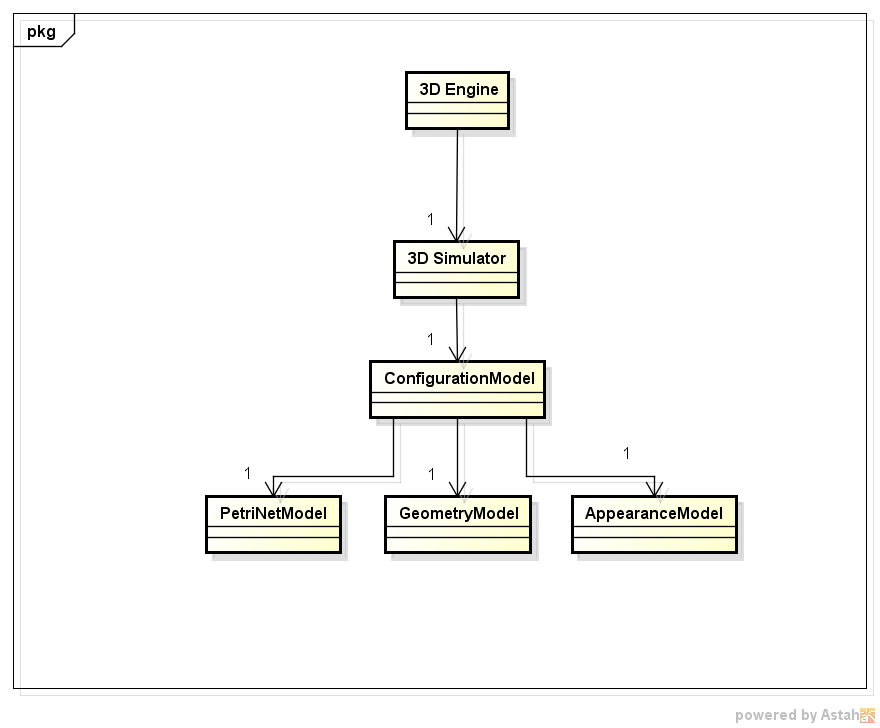
\includegraphics[width=0.5\textwidth]{image/domain_model.png}
  \caption{Domain model}
  \label{fig:domain-model}
\end{center}
\end{figure}

\newpage
\section{Petri net model}

\begin{figure}[htp]
\begin{center}
  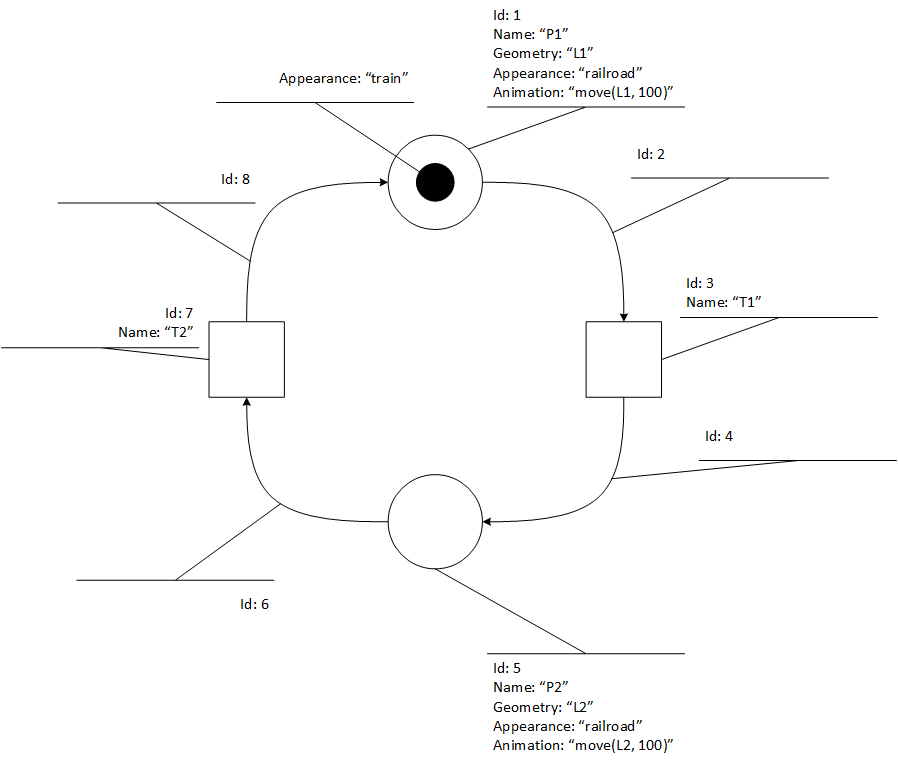
\includegraphics[width=0.6\textwidth]{image/example_petrinet.png}
  \caption{Example of an extended Petri net}
  \label{fig:extended_petrinet}
\end{center}
\end{figure}

Figure \ref{fig:extended_petrinet} shows an example of a particular extended Petri net. On this Petri net, there are two places (P1 and P2), two transitions (T1 and T2), and four arcs that link all the elements. Additionally, places can contain tokens. Moreover, the places contain additional information relevant for the simulator:
\begin{itemize}
\item A geometry label, to link the place to a geometry location
\item An appearance label, to link the place to a specific appearance, with shape, texture,...
\item An input place label, to indicate if the place is a special place that the user can click (for example to change \item the behaviour of the Petri net).
\item An animation label, to indicate how the 3D simulator should animate this place and the tokens contained in it.
\end{itemize}
A token also has an appearance label, in order to define its shape on the simulation.

\begin{figure}[htp]
\begin{center}
  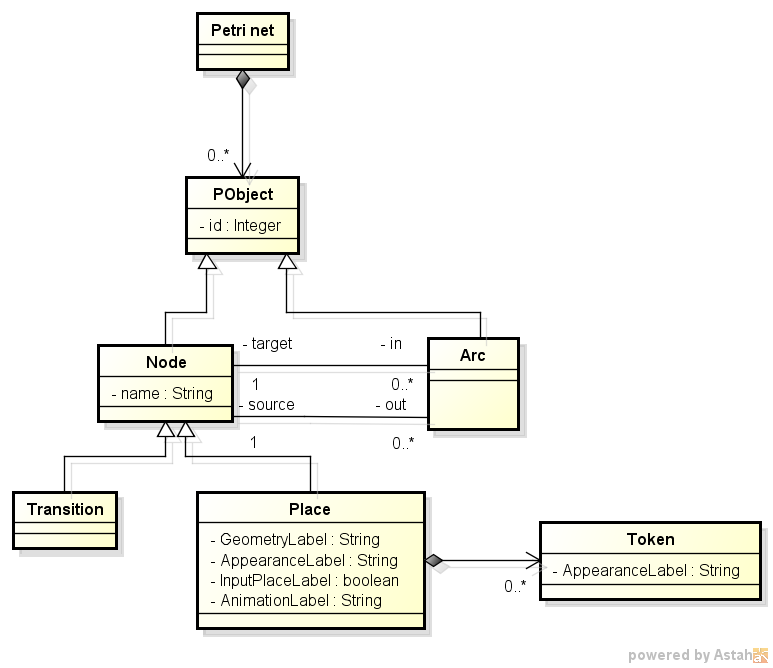
\includegraphics[width=0.7\textwidth]{image/petrinet_model.png}
  \caption{Petri net model}
  \label{fig:petrinet}
\end{center}
\end{figure}

\newpage
\section{Geometry model}


\begin{figure}[htp]
\begin{center}
  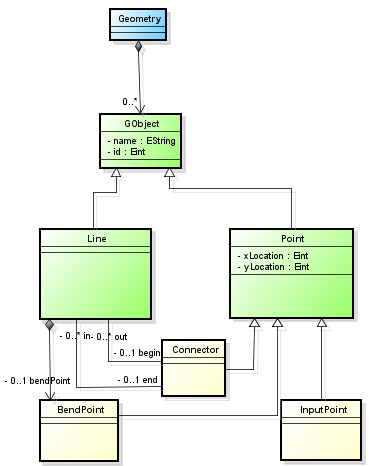
\includegraphics[width=0.6\textwidth]{image/geometry_model.png}
  \caption{Geometry Model}
  \label{fig:geometry_model}
\end{center}
\end{figure}

The diagram in Figure \ref{fig:geometry_model} describes the domain model associated with the geometry editor. The geometry editor can have an infinite number of GObjects, and each one has a name and an id. A GObject can either be a Point or a Line. A Point has a xLocation and an yLocation, which is the location of the Point in a 2D space.
Each Line has two connectors, one in each end of the line, and a bendPoint, which allows the user to bend the line to make curves. Connectors can have an infinite number of Lines connected to them. An InputPoint is a point that the user can interact with, to add or remove tokens during the simulation. 

Figure \ref{fig:extended_petrinet_geometry} is an example of how different lines can be connected in the Geometry Editor. The line with name L1 and id 1 has the two connectors C1 and C2 and the line L2 is also connected to the two connectors, C1 and C2. 


\begin{figure}[htp]
\begin{center}
  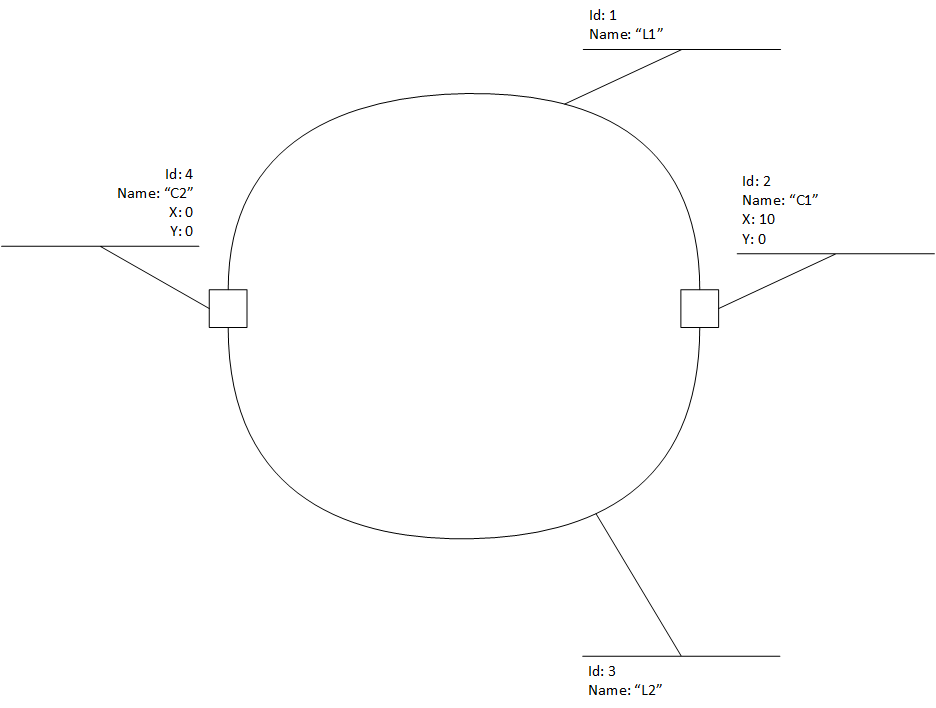
\includegraphics[width=0.6\textwidth]{image/example_petrinet_geometry.png}
  \caption{Example of a geometry}
  \label{fig:extended_petrinet_geometry}
\end{center}
\end{figure}

\newpage
\section{Appearance model}

The above diagram describes the domain model associated to the Appearance Editor described in the Project Definition. 
Each appearance model will have one or more objects of type AObject, each corresponding to an element in the Petri Net. The name attribute of each appearance object should be the same as the AppearanceLabel of its corresponding Petri Net object. Moreover, an appearance object has an associated 3DObject which is a file previously defined by the user and loaded in the Appearance Editor. Such a file can contain all or some of the following elements: 
\begin{itemize}
\item shape: sphere, cube, etc.
\item texture
\item color: red, green, black, etc.
\end{itemize}

The Appearance Model will in the end be structured as an XML file which will be used by the Configurator Editor.    

\begin{figure}[htp]
\begin{center}
  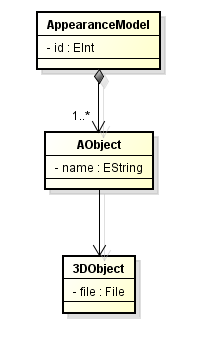
\includegraphics[width=0.2\textwidth]{image/appearance_model.png}
  \caption{Appearance Model}
  \label{fig:appearance_model}
\end{center}
\end{figure}

\newpage
\section{Configuration model}

The diagram in Figure \ref{fig:configuration_model} describes domain model associated to the Configuration Editor described in the Project Definition. It is quite simple because basically, a configuration model consists of the three files generated by the other editors (Petri net editor, Geometry editor, Appearance editor).
As each editor is generating an XML file, the configuration editor takes all these file as inputs. This can be seen in the UML diagram where a Configuration model has an association to each of the other models.
This model will be used by the Configuration Editor in order to create the final configuration XML file which will be provided to the simulator.

\begin{figure}[htp]
\begin{center}
  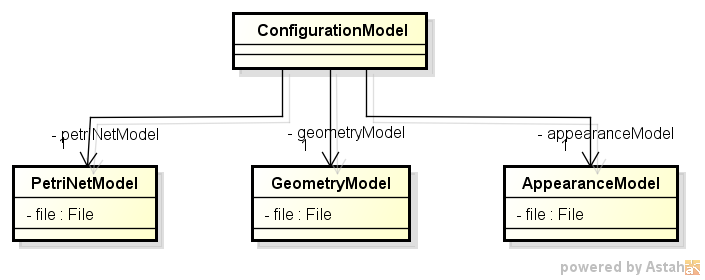
\includegraphics[width=0.6\textwidth]{image/configuration_model.png}
  \caption{Configuration Model}
  \label{fig:configuration_model}
\end{center}
\end{figure}

\newpage
\section{3D Simulator model}

The UML diagram of the Simulator visualizes how the Simulator is dependant on the jMonkey 3D framework, that is used to run the simulation. Also, the Simulator needs a configuration file in order to function. The configuration file is used to specify what the SObjects look like and how they behave; SObjects have an 'id' and a 'name' in order to properly link them with the configuration. The SObjects can be used to create Places that have Tokens. There can be as many Places as desired, and as many Tokens on each Place as desired, but a Token can only have one Place.

\begin{figure}[htp]
\begin{center}
  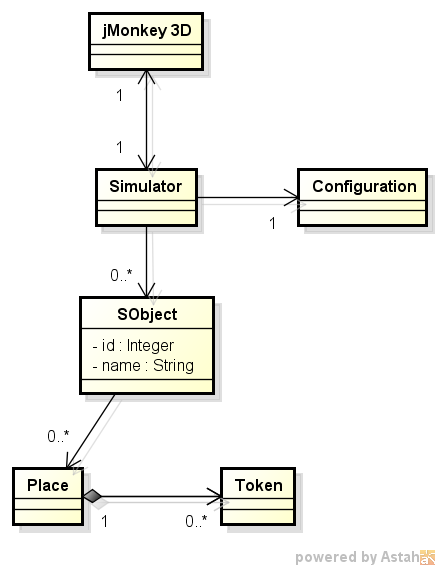
\includegraphics[width=0.4\textwidth]{image/simulator_model.jpg}
  \caption{Simulator Model}
  \label{fig:simulator_model}
\end{center}
\end{figure}

\printindex



\end{document}

